\documentclass[a4paper,12pt,singlespacing]{article}
% Arquivo de configurações do modelo
\usepackage[T1]{fontenc}
\usepackage[utf8]{inputenc}
\usepackage[lmargin=2cm, rmargin=2cm, tmargin=2.5cm, bmargin=2.5cm]{geometry}
% \usepackage[brazil, brazilian]{babel}
\usepackage[style=abnt]{biblatex}
\usepackage{csquotes, graphicx, xcolor, comment, enumerate, multirow, multicol, titlesec, amsmath, amsthm, amsfonts, amssymb, dsfont, mathtools, blindtext, ragged2e, array, enumitem, tikz, bbding, pifont, wasysym, amssymb, hyperref, titling}
\newcommand{\cmark}{\ding{51}}
\newcommand{\xmark}{\ding{55}}

\tolerance=1
\emergencystretch=\maxdimen
\hyphenpenalty=10000
\hbadness=10000

\usepackage{helvet}
\renewcommand{\familydefault}{\sfdefault}

\usepackage{setspace}
\setlength{\JustifyingParindent}{1.25cm}
\setlength{\RaggedRightParindent}{0pt}
\setlength{\parskip}{6pt}

\usepackage{fancyhdr}
\pagestyle{fancy}
\fancyhf{}
\lhead{}
\rhead{}
\rfoot{\small\thepage}
\renewcommand{\headrulewidth}{0pt}

\titlespacing*{\section}{0pt}{6pt}{0pt}
\titlespacing*{\subsection}{0pt}{6pt}{0pt}
\titlespacing*{\subsubsection}{0pt}{6pt}{0pt}

\renewcommand{\thesection}{\arabic{section}.}
\renewcommand{\thesubsection}{\arabic{section}.\arabic{subsection}.}
\renewcommand{\thesubsubsection}{\arabic{section}.\arabic{subsection}.\arabic{subsubsection}.}

\titleformat{\section}{\normalsize\bfseries}{\makebox[1.25cm][l]{\thesection}}{0pt}{}
\titleformat{\subsection}{\normalsize\bfseries}{\makebox[1.25cm][l]{\thesubsection}}{0pt}{}
\titleformat{\subsubsection}{\normalsize\bfseries}{\makebox[1.25cm][l]{\thesubsubsection}}{0pt}{}

\usepackage{textcase}
\usepackage[font=small, labelsep=endash, textfont=bf, labelfont=bf, aboveskip=6pt, belowskip=-6pt, tablename=TABELA, figurename=FIGURA]{caption}
\usepackage[font=small, labelsep=endash, textfont=bf, labelfont=bf, aboveskip=6pt, belowskip=3pt, labelformat=simple]{subcaption}

\renewcommand{\thetable}{\arabic{table}}
\renewcommand{\thefigure}{\arabic{figure}}
\renewcommand{\thesubfigure}{\arabic{subfigure}}
\renewcommand{\thesubtable}{\arabic{subtable}}

\addbibresource{ref.bib}


% Utilizado para correções e comentários. Vá para 'util.tex' para saber mais.
\usepackage[normalem]{ulem}
\usepackage{color}
\usepackage[T1]{fontenc}

% Uso: \comando{texto}, onde 'comando' pode ser 'entra', 'sai', 'rever', 'todo', ou \comando[nota adicional]{texto}

\newcommand{\entra}[2][]{
   {\color{blue}#2}
   \ifx&#1&
      {}
    \else
      \footnote{{\color{blue}(entra):} #1}
    \fi
}

\newcommand{\sai}[2][]{
   {\color{black}\sout{#2}}
   \ifx&#1&
      {}
    \else
      \footnote{{\color{black}(sai):} #1}
    \fi
}

\newcommand{\rever}[2][]{
   {\color{magenta}#2}
   \ifx&#1&
      {}
    \else
      \footnote{{\color{magenta}(rever):} #1}
    \fi
}

\newcommand{\todo}[2][]{
   {\color{red}[ \textbf{TODO}: \textit{#2} ]}
   \ifx&#1&
      {}
    \else
      \footnote{{\color{red}(todo):} #1}
    \fi
}

\newcommand{\etal}{{\sl et~al.}}

\newcommand{\<}{\textrm{<}}
\renewcommand{\>}{\textrm{>}}


% Aqui devem ser inseridas as informações sobre o trabalho
    % Título:
    \title{PROJECT DESIGN III: PJD 301B}
    % Alunos e orientadores:
    \author{DESIGN DOCUMENTATION}
    % E-mails dos integrantes:
    \def\emails{e-mail do aluno 1, e-mail do aluno 2, e-mail do aluno 3, e-mail do Orientador, e-mail do Coorientador}

% Na pasta 'artigo' estão as respectivas seções que devem constar no trabalho. Lá deve ser inserido todo o conteúdo.

% Para referências, consulte 'ref.bib' e saiba mais. Na seção de Referencial Teórico, são exemplificadas as formas de se fazer uma citação.

\begin{document}
    {\centering
		\begin{figure}[!ht]
			\centering
			
\includegraphics[scale=0.15]{./tut_logo.png}
		\end{figure}

        \setlength{\parskip}{0pt}
		FACULTY OF INFORMATION \\ AND \\  COMMUNICATION TECHNOLOGY

        \setlength{\parskip}{18pt}
		NATIONAL DIPLOMA: COMPUTER SYSTEMS ENGINEERING

        \setlength{\parskip}{18pt}
        \textbf{ \thetitle }
        \setlength{\parskip}{12pt}

        \theauthor

        \setlength{\parskip}{6pt}
        % \footnotesize{\emails}

    }


    \clearpage  % Certification ended, now start a new page
    \tableofcontents
    \clearpage  % Certification ended, now start a new page


    \justifying

    % \section*{Resumo}

\noindent
% Resumo
Apresentar o texto do resumo em um único parágrafo (bloco único, sem recuo à esquerda). O resumo deve apresentar, de forma breve, o tema e sua importância, os objetivos, o marco teórico principal, a metodologia e os resultados alcançados. Logo, se apresenta no resumo uma visão clara do conteúdo e das conclusões do trabalho destacando os pontos relevantes. O resumo deve ser apresentado contendo entre 200 e 300 palavras. O texto do resumo e das palavras-chave são apresentados em fonte arial tamanho 12, com alinhamento do texto justificado e espaçamento de parágrafo em 6 pt antes e 6 pt depois. O espaçamento entre linhas é simples. Logo após o resumo são apresentadas as 3 (três) palavras-chave que representam o conteúdo do trabalho. Os termos “Resumo” e “Palavraschave” são apresentados em negrito e são alinhados à esquerda. Após o termo “Palavraschave” é inserido o sinal de dois pontos “:” para identificar o início das palavras selecionadas. As palavras são separadas entre si por ponto-e-vírgula “;” e após a última é inserido o ponto final “.”.

\noindent\textbf{Palavras-chave:}
% Palavras-chave
Palavra 1; Palavra 2; Palavra 3.


    \subsection{Introduction}

% \subsubsection{\textit{Purpose}}
The following document outline all design documentation of the smart livestock monitoring
System. This document is separated in section, you can jump to any specific section you want to learn more
about related to the livestock monitoring system. You are advice to read this document if you want to
learn more about the design principle and choices of the livestock monitoring system. The information on this document will
enable you to not only understand the system but will tell you how to trouble shoot the system if anything went
wrong and also extend the functionality of the system if you so choose to.

\subsubsection{\textit{Scope}}
The document will cover design consideration, Assumptions, goals and guideline. It will give you enough information
about Architectural strategies, System architectural and Functional flow of the livestock monitoring system.

\subsubsection{\textit{Audience}}
The design documentation is for anyone who want to learn more about the livestock monitoring system,
How it is design from ground up and how they can extend the system to solve other problem. This document it also
good for any engineers who want to replicate the system on their own.

% Apresentar o texto do objetivo. Em caso de utilização de lista, eis um exemplo:
% \begin{itemize}[noitemsep, topsep=0pt]
%     \item item 1;
%     \item item 2;
%     \item item 3.
% \end{itemize}


    \subsection{Systems overview}

The smart livestock monitoring system track livestock using ESP32 Micro controller. One ESP32 per
each livestock that contain a unique identify (UID) that will enable the system to count the total
livestock at a given time. A web sever connect to a database take the information sends sends by
the Micro controller and store it to a database.

The Micro controller is  being package to a case with a battery. The band that
cover the animal is a solar panel that charge the
battery so that it does not die quick. The case is that package the microcontroller is strong enough
to resist hard weather condition


    \section{Design considerations (1/2 page)}

This section describes many of the issues which need to be addressed or
resolved before attempting to devise a complete design solution.


    \section{Assumptions and dependencies (1/2 page)}

Describe any assumptions or dependencies regarding the software and hardware and their use. These may concern such issues as related software and hardware, end user characteristics etc
\subsection{Related software and hardware}
Describe the relative software and hardware.
\subsection{End-user characteristics}
Possible and/or probable changes in functionality
\subsection{General Constraints}

Describe any global limitations or constraints that have a significant impact on the design of the system's software (and describe the associated impact). Such constraints may be imposed by any of the following (the list is not exhaustive):

    • Hardware or software environment
    • End-user environment
    • Availability or volatility of resources
    • Other requirements described in the requirements specification


    \section{Goals and guidelines (1/2 page)}

Describe any goals, guidelines, principles, or priorities which dominate or embody the design of the system's software. Such goals might be:

    • The KISS principle ("Keep it simple stupid!")
    • Emphasis on speed versus memory use
    • Working, looking, or "feeling" like an existing product

For each such goal or guideline, unless it is implicitly obvious, describe the reason for its desirability. Feel free to state and describe each goal in its own sub-subsection if you wish.


    \section{Modelagem do Sistema}

Apresentar o texto referente a modelagem do sistema. Esta seção aplica-se, exclusivamente, aos projetos interdisciplinares que remetem ao desenvolvimento de sistemas, como solução para o problema identificado, foco do presente projeto.

Deverão ser apresentados os principais diagramas que representam o projeto. A escolha de quais diagramas serão usados e apresentados ficará a cargo de cada orientador. Entretanto, sugere-se que sejam apresentados, no mínimo, o Diagrama de Casos de Uso, O Diagrama Entidade-Relacionamento e o Diagrama de Classes.

    \section{Sistema}

Apresentar o texto e as imagens referente ao sistema desenvolvido explicitando as
funcionalidades desenvolvidas.

% Exemplo de inserção de figura com subfiguras
\begin{figure}[htbp]
\centering
    \begin{subfigure}[b]{7cm}
        \centering
        % Primeira subfigura
        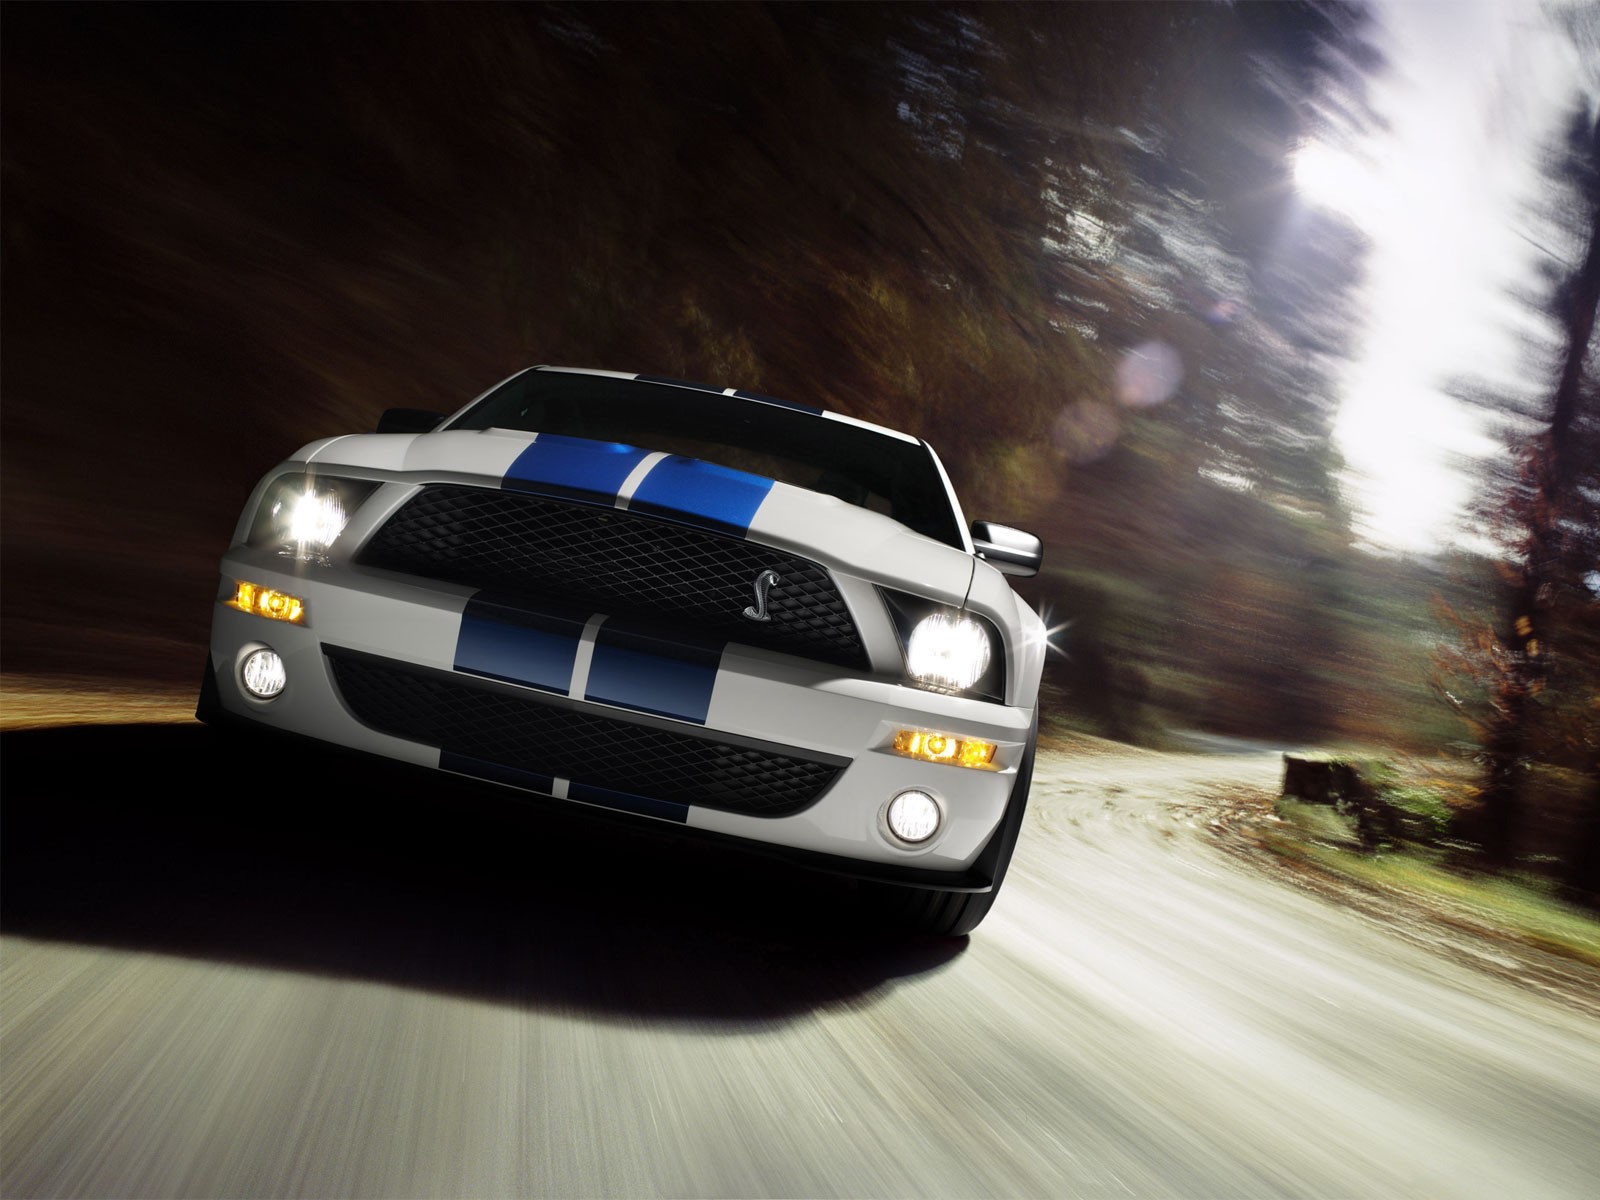
\includegraphics[width=7cm]{anexos/sub1fig2.jpg} % URI da subfigura
        \subcaption{
        % Legenda da subfigura
        Carro branco.
        }
        \label{fig2:sub1}
    \end{subfigure}
\quad
    \begin{subfigure}[b]{7cm}
        \centering
        % Segunda subfigura
        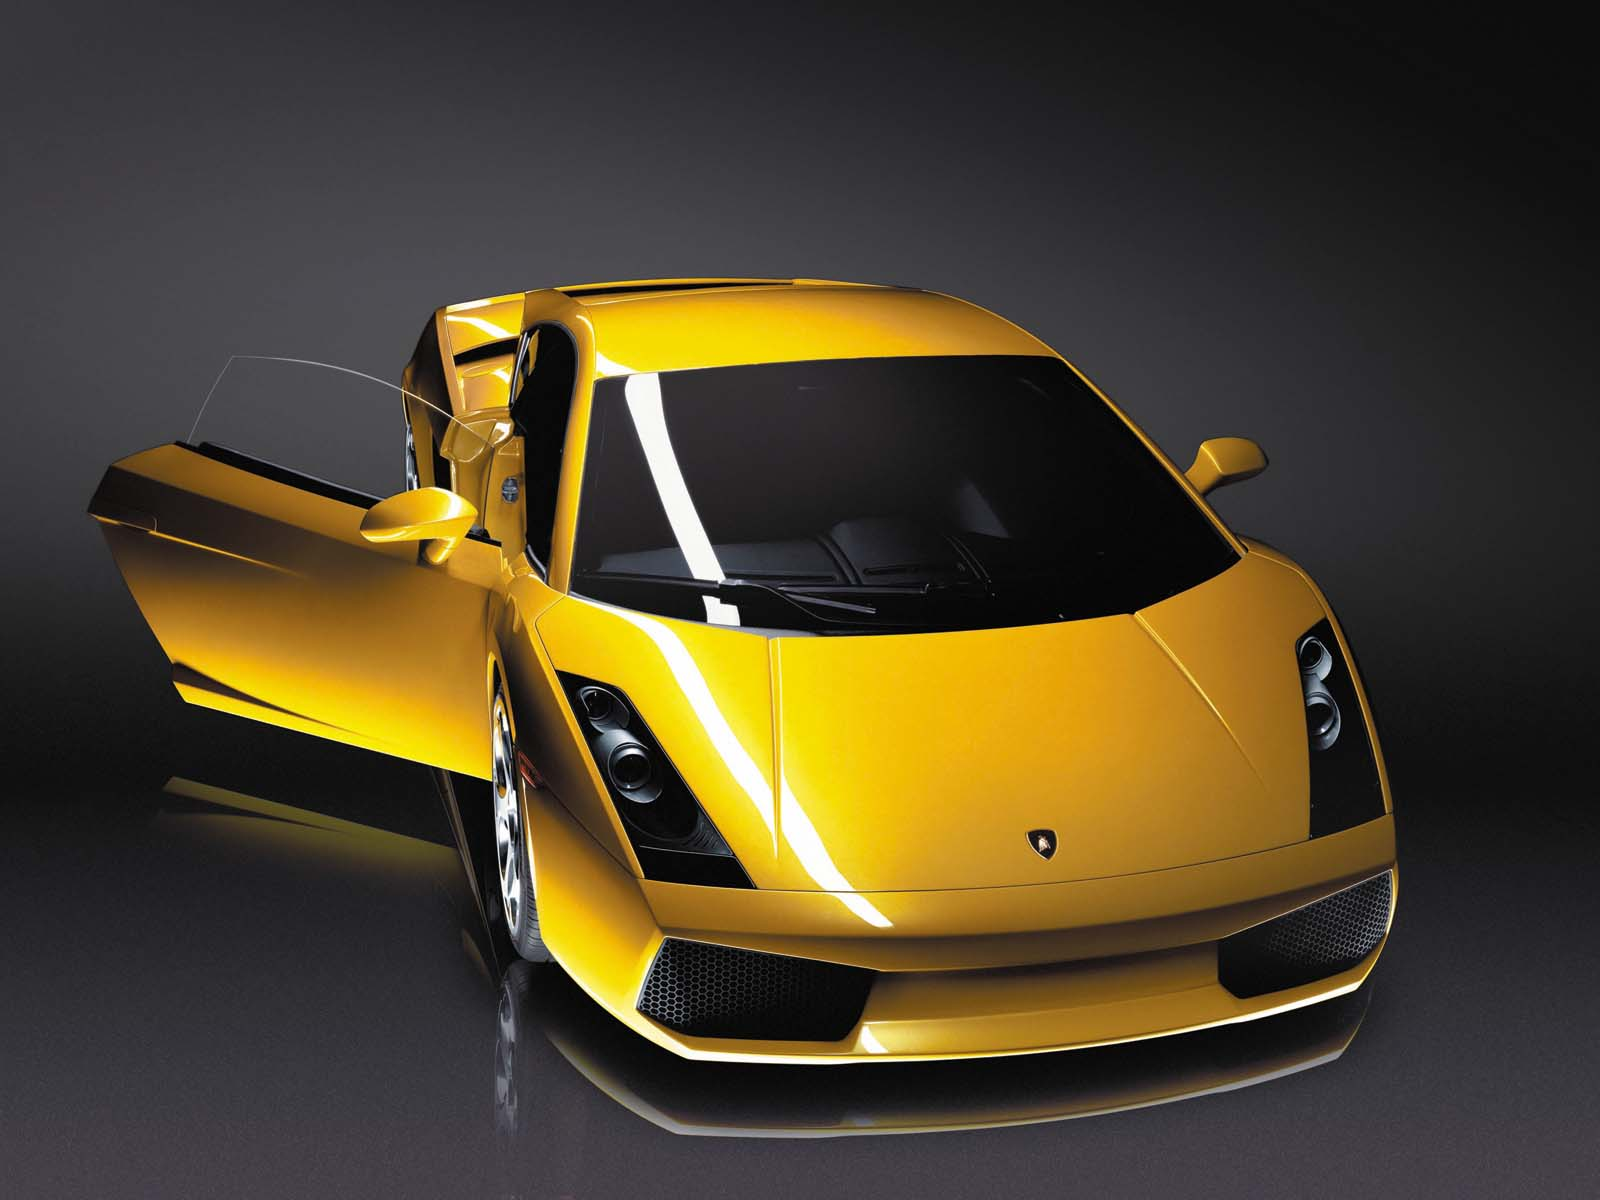
\includegraphics[width=7cm]{anexos/sub2fig2.jpg} % URI da subfigura
        \subcaption{
        % Legenda da subfigura
        Carro amarelo.
        }
        \label{fig2:sub2}
    \end{subfigure}
\caption{
Legenda da figura.
}
\label{fig:fig2} % Tag para referência
\end{figure}

    \section{Considerações Finais}

Apresentar o texto das considerações finais de forma que os resultados obtidos sejam reavaliados em relação aos objetivos e a pergunta de estudo (questão problema). É necessário atentar e verificar se os resultados obtidos respondem a pergunta de estudo e se os objetivos propostos (seção 1.1) foram alcançados. Caso estes não tenham sido alcançados se faz necessário apresentar as dificuldades encontradas e o motivo pelo qual não foram alcançados.

Ressalta-se que o texto aqui apresentado é breve, conciso e coerente. Logo, uma conclusão apresentada não pode se contrapor a outra.

    \section{Referências}

    \raggedright
    \printbibliography[heading=none]
\end{document}
